\documentclass{article}

% Language setting
% Replace `english' with e.g. `spanish' to change the document language
\usepackage[english]{babel}
\usepackage[compat=1.1.0]{tikz-feynman}
\usepackage{booktabs}
\usepackage{amsthm}
\usepackage{algorithm}
\usepackage{algpseudocode}
\usepackage{graphicx}
\usepackage{subcaption}
\usepackage{epigraph}
\usepackage{csquotes}
\usepackage{verbatim}
\usepackage{markdown}
\usepackage{csvsimple}
% Set page size and margins
% Replace `letterpaper' with `a4paper' for UK/EU standard size
\usepackage[letterpaper,top=2cm,bottom=2cm,left=3cm,right=3cm,marginparwidth=1.75cm]{geometry}

% Useful packages
\usepackage{amsmath}
\usepackage{graphicx}
\usepackage[colorlinks=true, allcolors=blue]{hyperref}

\newtheorem{theorem}{Theorem}[section]
\newtheorem{lemma}[theorem]{Lemma}


\begin{document}

\begin{titlepage}
    \centering
    
    \vspace*{\fill}
    
    \textbf{\LARGE [Re] Discovering Symbolic Models from Deep Learning with Inductive Biases}\\
    \vspace{0.5cm}
    \hrule % Horizontal line
    \vspace{0.5cm}
    \textbf{\Large Final Project}
    
    \vspace{3cm}
    
    \textbf{University of Cambridge}\\
    \hrule % Horizontal line
    \vspace{0.5cm}
    \text{Department of Physics}
    
    \vspace{0.5cm}
    
    \textbf{Prepared by:}\\
    \text{Sabahattin Mert Daloglu}\\
    \vspace{0.5cm}
    \textbf{Supervised by:}\\
    \text{Miles Cranmer}\\
    \vspace{0.5cm}
    \text{Word Count: XXXX}
    \vspace{1cm}
    
    \today
    
    \vspace*{\fill}
\end{titlepage}

\newpage % Start the main content on a new page
%%%%%%%%%%%%%%%%%%%%%%%%%%%%%%%%%%%%%%%%%%%%%%%%%%%%%%%%%%%%%%%

\section{Abstract}
This paper is a reproduction and analysis of the novel work demonstrated in \textbf{Discovering Symbolic Models from Deep Learning with Inductive Biases} by Cranmer et. al. Both explicit -architecture bottlenecks-, and implicit -regularization- based inductive biases are utilized to induce sparse latent representations of edge model of the Graph Networks (GNs) trained on minimizing the difference between the node model outputs and the simulated instantaneous acceleration of the particles in physical systems. Later, symbolic regression is applied to the sparsed representation of the edge embeddings to extract the physical relations between particles. As found by Cranmer et. al. the correct known force law equations are recovered for the Newtonian, spring, and charge systems in 2 and 3 dimensions. The analysis of models with different regularization methods -L1, Kullback-Leiber and Bottleneck- are compared in their successes in predicting the true force of the system and recovering the known physical equations fitted by symbolic regression. As an extension, a scheduler on the L1 regularization coefficient with a linear increase until the mid-point of the training than linear decrease until the end of training iterations was studied. The purpose of this extension was to explore the trade-off between the expressiveness of the latent space in the early stages of training and the sparsity of the learned message embeddings that are expected to converge to the true number of dimensions of the physical system. A scheduler on the L1 regularization yielded better sparsity and performance of the model.



\section{Introduction}

While deep learning models are very good at learning the labels of the data represented in high-dimensional space, they are commonly referred to as black-box models noting their lack of interpretability. On the other hand, symbolic closed-form (explain what I mean by closed-form) expressions, explicitly demonstrate the correspondence of the input variables with the output directly. The work reproduced in this paper is a notable attempt to demonstrate the intersection of these two in the pursuit of making black-box deep learning models more interpretable to extract the physical intuition behind these architectures.

Since its increase in use in scientific papers with the introduction of the Eureqa software, symbolic regression has been used to extract analytical functions from a large dataset of experimental data. Although adventagous for interpretability and expressiveness, the brute-force search of the solution space is a major drawback. Evolutionary algorithms such as genetic algorithms are used to iteratively search the solution space. The selection of the best solution is based on the fitness function and results are manipulated based on genetic operations such as reproduction, crossover, mutation mimicking the process of natural selection. The number of iterations to converge to a solution increases exponentially with the given dimension of the operator space and inputs. The use of GNs comes handy due to their naturally separable internal structure which is convenient for the Newtonian problems under study. This separability allows us to apply symbolic regression to smaller sub-sections of the model and hence reducing the iterations of the solution space search. These separate symbolic expressions can be later combined to give an overall expression of the model learned by the whole GN. This extracted symbolic equation generalizes better than the GN model to a new unseen test data.

\section{Theory and Framework}

A natural starting point of discussion is a brief overview of the message-passing graph networks used in this study. A general nomenclature of graphs is given by {cite GN paper} and used as a reference in this paper. A graph is defined by a set of nodes $V = \{\textbf{v}_i\}_{i=1:N^v}$ with set size $N^v$ and edges $E = \{\textbf{e}_k, r_k, s_k\}_{k=1:N^e}$ with set size $N^e$. Each $\textbf{v}_i$ is a node feature vector of dimension $L^v$. Similarly, each $\textbf{e}_k$ is an edge feature vector with dimensions $L^e$ corresponding to the sender node index $s_k$ and receiver node index $r_k$. This graph structure will be the input data type for the GN model and is illustrated in \ref{fig:graph}.

\begin{figure}[htbp]
    \centering
    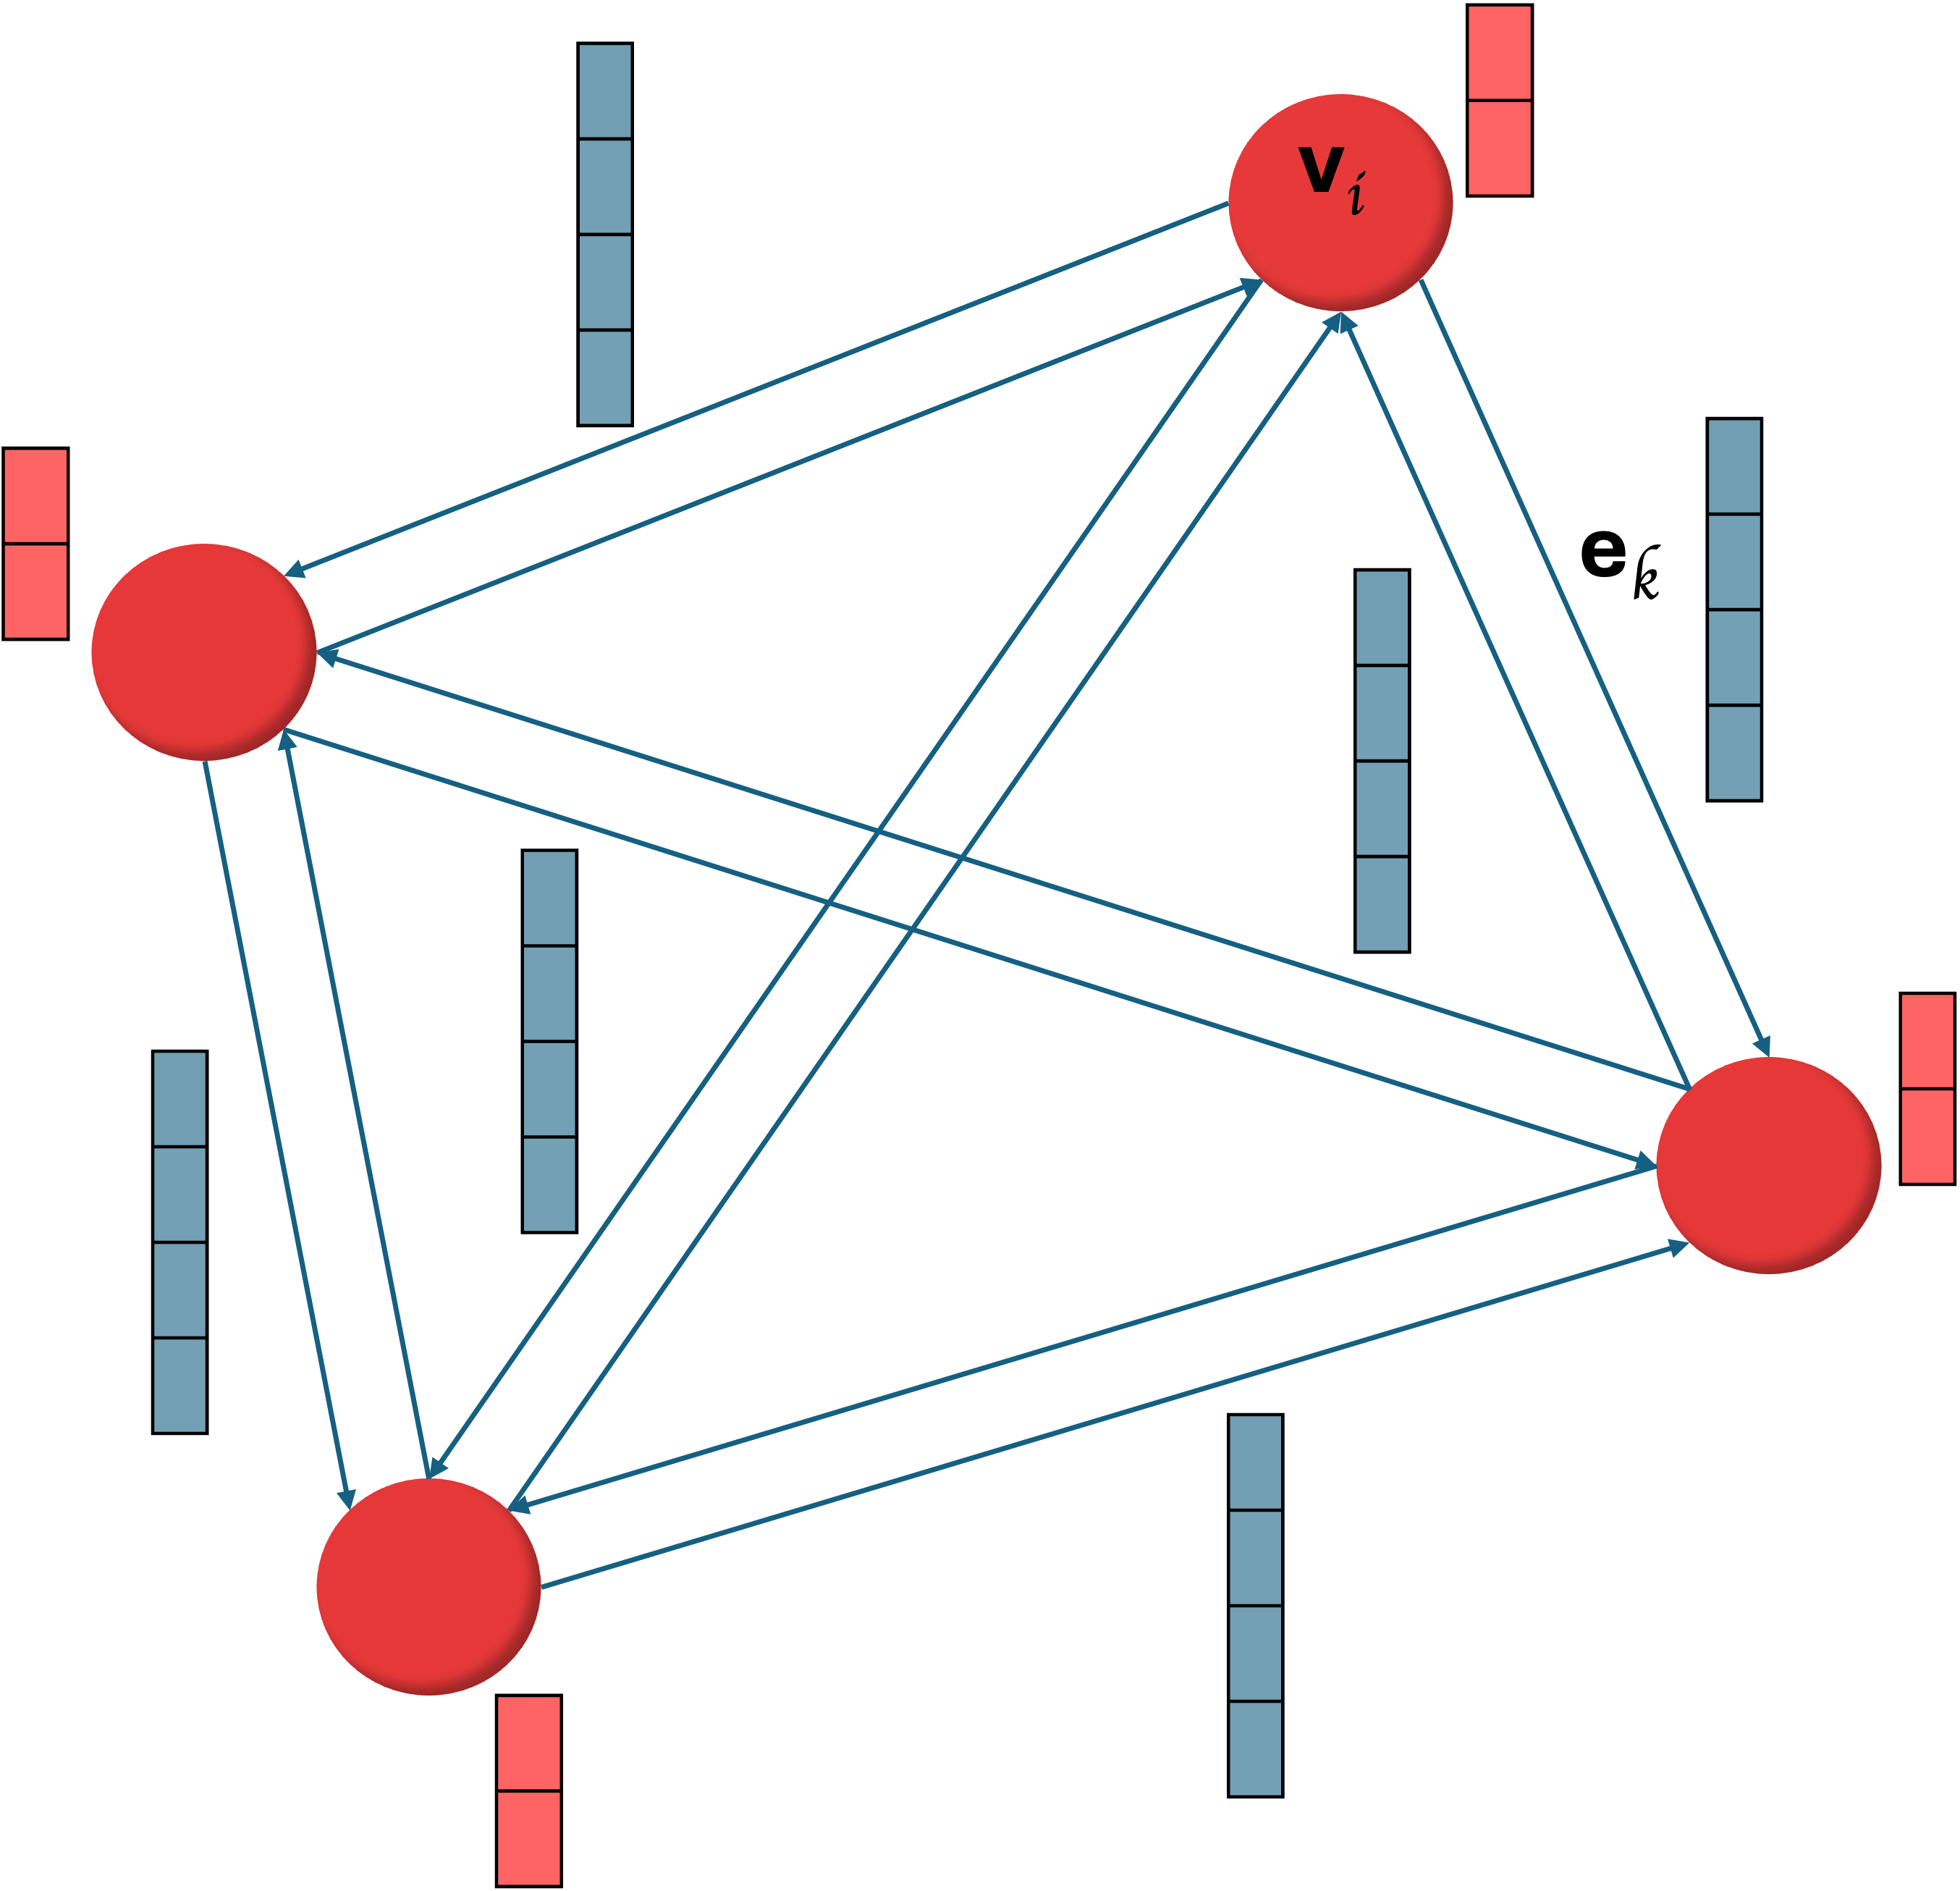
\includegraphics[width=0.5\textwidth]{images/graph.png}
    \caption{Graph structure of the GN model.}
    \label{fig:graph}
\end{figure}

Graph networks consist of three separable components that are the edge model $\phi^e$, the node model $\phi^v$, and the global model $\phi^u$ as well as the intermediate step of aggregation. These three models are used consecutively to predict the next state of the graph defined by set of  $V'$ nodes and $E'$ edges. The models are described below:

\begin{itemize}
    \item \textbf{Global Model $\phi^u$}: This model is used to update some arbitrary global metric of the system represented in graph such as the gravitational field of the system under study{cite GNN paper}. This is a graph-level attribute and is generally used for predicting dynamical systems. Since, each time step (snapshot) of graph is treated as independent with considering instantaneous forces and accelerations, this model is not used in the original paper.
    \item \textbf{Edge Model $\phi^e$}: A function $\phi^e$ with mapping $\mathbb{R}^{L^v} \times \mathbb{R}^{L^v} \to \mathbb{R}^{L^{e'}}$, usually consisting of multilayer perceptions (MLPs), that intakes two node feature vectors that are connected by an edge and outputs an edge embedding. The updated edge vector is found by $\textbf{e}_k' = \phi^e(\textbf{e}_k) = \phi^e(\textbf{v}_r, \textbf{v}_s)$. This edge embedding contains the information about the interaction of the nodes (particles in this study) and is expected to correspond to pairwise force between connected nodes/particles in the system.
    \item \textbf{Aggregation}: This is an intermediate updating step which does not consist of MLPs but only a summation of the edge embeddings. This corresponds to the net force calculation in Newtonian systems. For a given receiving node, all the edges its connected to has a corresponding edge embedding after the edge model is applied. These messages are summed to give the aggregated edge embedding of the receiving node: $\bar{\textbf{e}}_i' = \sum_{k \in \{1:N^e \mid r_k = i\}} \textbf{e}_k'$ where $\bar{\textbf{e}}_i'$ is the aggregated edge vector of the receiving node $r_i$. 
    \item \textbf{Node Model $\phi^v$}: A function $\phi^v$ with mapping $\mathbb{R}^{L^v} \times \mathbb{R}^{L^{e'}} \to \mathbb{R}^{L^{v'}}$, usually consisting of multilayer perceptrons (MLPs), that intakes the aggregated edge embeddings corresponding to a receiving node and its node features. The output of the node model is the prediction of the instantaneous acceleration of the receiving node/particle. The GN model used in this study is a node-focused GN (cite GN paper), which means the output of the node model is used in loss calculation by comparing against the ground truth acceleration values. This part of the model corresponds to the Newton's second law of motion where the acceleration on a body is computed via dividing the net-force (aggregated edge embeddings) by the mass of the body (node feature).
\end{itemize}

The separable structure of the message-passing Graph Network, and the correspondence of the edge-node models to the force-acceleration calculations of the Newtonian systems under study is the cornerstone of the inductive biases introduced in the paper. 

The next important inductive bias is the regularization of the edge embeddings to implicitly encourage sparsity in the learned edge vectors. This is achieved by incorporating either L1 regularization or a KL-divergence term into the loss function. It is important to recognize that through this regularization, we are aiming to bias the edge embeddings to converge to the true number of dimensions of the forces in the system, without explicitly providing the true forces or the number of dimensions. Consequently, the sparsely represented edge embeddings are learned as a linear transformation of the true forces in an unsupervised manner, as the training process is based on minimizing the acceleration prediction error. A rough mathematical explanation is given in the main paper, here we sketch a more detailed proof why this is the case:

To mathematically prove that the learned edge embeddings are linear transformations of the true forces, consider the following:


\begin{enumerate}
    \item \textbf{Definitions and Assumptions}:
    \begin{itemize}
        \item Let \( \mathbf{F}_{\text{true}} \) represent the true force vector in the system.
        \item The edge model \( \phi^e \) learns an embedding \( \mathbf{e}_k' \) from node features \( \mathbf{v}_r \) and \( \mathbf{v}_s \) connected by an edge \( k \).
        \item The regularization term (either \( L_1 \) or KL-divergence) in the loss function minimizes the dimensionality of \( \mathbf{e}_k' \), promoting sparsity.
        \item The training minimizes the loss function 
        \[
        \mathcal{L} = \|\mathbf{a}_{\text{pred}} - \mathbf{a}_{\text{true}}\|^2 + \lambda \|\mathbf{e}_k'\|,
        \]
        where \( \mathbf{a}_{\text{pred}} \) is the predicted acceleration, \( \mathbf{a}_{\text{true}} \) is the true acceleration, and \( \lambda \) is the regularization coefficient.
    \end{itemize}

    \item \textbf{Newton's Second Law}:
    \begin{itemize}
        \item According to Newton's second law,
        \[
        \mathbf{a}_{\text{true}} = \frac{\mathbf{F}_{\text{true}}}{m},
        \]
        where \( m \) is the mass of the particle.
    \end{itemize}

    \item \textbf{Model Prediction}:
    \begin{itemize}
        \item The model learns to predict \( \mathbf{a}_{\text{pred}} \) such that 
        \[
        \mathbf{a}_{\text{pred}} \approx \mathbf{a}_{\text{true}}.
        \]
    \end{itemize}

    \item \textbf{Edge Embedding and Force Relationship}:
    \begin{itemize}
        \item Since the model aims to minimize the loss function \( \mathcal{L} \), the learned edge embedding \( \mathbf{e}_k' \) must be related to the true force \( \mathbf{F}_{\text{true}} \) in a way that minimizes the prediction error.
        \item Given the regularization term, \( \mathbf{e}_k' \) is encouraged to be sparse, implying that it captures the most significant components of the true force.
    \end{itemize}

    \item \textbf{Linear Transformation}:
    \begin{itemize}
        \item To minimize the loss function effectively, \( \mathbf{e}_k' \) must be a linear transformation of \( \mathbf{F}_{\text{true}} \). This can be expressed as:
        \[
        \mathbf{e}_k' = \mathbf{W} \mathbf{F}_{\text{true}} + \mathbf{b},
        \]
        where \( \mathbf{W} \) is a learned weight matrix and \( \mathbf{b} \) is a bias vector.
    \end{itemize}

    \item \textbf{Detailed Proof}:
    \begin{itemize}
        \item Let \( \mathbf{f}_i \) be the net force on the \( i \)-th body, calculated as the sum of individual forces \( \mathbf{f}_k \) acting on it:
        \[
        \mathbf{f}_i = \sum_{r_k=i} \mathbf{f}_k.
        \]
        \item Assume the Graph Network predicts accelerations perfectly. Then, if we ignore the mass of the target body, the predicted net force for body \( i \) can be approximated as:
        \[
        \hat{\mathbf{f}}_i \approx \mathbf{a}_i = \sum_{r_k=i} \mathbf{f}_k = \phi^v(\mathbf{v}_i, {\bar{\mathbf{e}}_i}),
        \]
        This is true for any number of bodies. For a two-body system with a single interaction, the predicted net force can be approximated as:
        \[
        \hat{\mathbf{f}}_i = \mathbf{f}_{k,r_{k}=i} = \phi^v(\mathbf{v}_i, \mathbf{e'}_{k,r_{k}=i}),
        \]
        The two-body system can be summed over the number of bodies to get the multi-body system's expression:


        \[
        \sum_{r_k=i} \mathbf{f}_k = \sum_{r_k=i} \phi^v(\mathbf{v}_i, \mathbf{e'}_{k}) = \phi^v(\mathbf{v}_i, \sum_{r_k=i} {\mathbf{e'}_{k}}).
        \]

        From this, we can see that  \( \phi^v \) has to be a linear operation. To find how this relates to the edge embeddings, we take the inverse of \( \phi^v \) and apply it to the true forces \( \mathbf{F}_{\text{true}} \):
        \[
        \mathbf{e'}_{k} = (\phi^v(\mathbf{v}_i, \cdot))^{-1}(\mathbf{f}_k).
        \]

        Since, \( \phi^v \) is a linear operation, its inverse is also a linear operation. Moreover, \( \phi^v \) is only invertible if the output of \( \phi^v \) and \( \bar{\mathbf{e'}_{i}} \) have the same number of dimensions. Since, previously we assumed that \( \phi^v \) perfectly predicts the instantaneous accelerations, this is only the case if the number of dimensions of \( \bar{\mathbf{e'}_{i}} \) is equal to the true dimensions of the system. Therefore, by introducing regularization to the loss function, and sparsing the edge embeddings, we can ensure that \( \phi^v \) is invertible, hence the learned edge embeddings \( \mathbf{e}_k' \) are linear transformations of the true forces \( \mathbf{f}_k \).

    \end{itemize}

    \item \textbf{Conclusion}:
    Under the assumption that the model predicts the instantaneous accelerations perfectly, and the regularization is applied to the edge embeddings such that they are sparse and correspond to the true number of dimensions, then it is shown that the edge embeddings are linear transformations of the true forces.
\end{enumerate}


In the Symbolic Regression section, we confirm that this holds true by fitting a symbolic regression on the sparsed edge embeddings and comparing the resulting equation to the true force equations of the Newtonian system. If the recovered equation is the linear transformations of the true forces as shown for the spring system in \ref{eq:spring_2d_pred}, then the model is able to learn the forces in the system and the proof above is correct experimentally as well.


\begin{equation}
    \mathbf{F}_{\text{spring}} = -2(\Delta x, \Delta y) \cdot (\frac{r - 1}{r})
    \label{eq:spring_2d_true}
\end{equation}

\begin{equation}
    \phi^e_1 = -2 \mathbf{a} \cdot (\Delta x, \Delta y) \cdot (\frac{r - 1}{r})+b
    \label{eq:spring_2d_pred}
\end{equation}



The final inductive bias for this study is the choice of the Adam optimizer which is another implicit regularization in the loss function as discussed by Simons {cite}. The choice of optimizer and loss function provides a bias for the learning process and the loss curve. The choice of Adam optimizer with learning rate schedules is well-motivated by the state-of-the-art research on Graph Neural Networks (cite).



\section{Scope of Reproducibility}

In this paper, the following items from the original papers are aimed to be reproduced:

\begin{enumerate}
    \item Claim 1: Implementation of the Graph Network architecture with a single message passing step.
    \item Claim 2: Train the Graph Network using the selected hyperparameters and regularization techniques on the following 2-dimensional systems: spring, charge, \( r^{-1} \), and \( r^{-2} \).
    \item Claim 3: Achieve a sparse latent representation of the learned messages, preferably corresponding to the true number of dimensions.
    \item Claim 4: Test the performance of L1 regularization, KL-divergence, and Bottleneck regularization on the learned messages.
    \item Claim 5: Compare the performance of the bottleneck model with the regularizer models.
    \item Claim 6: Learn a symbolic model from the sparse representation of the learned messages by applying symbolic regression using PySR to approximate the message embeddings.
    \item Claim 7: Recover the linear transformation of the known physical laws of the spring, charge, and Newtonian systems.
    \item Claim 8: Test the performance of the symbolic models on the test datasets and confirm symbolic equations generalize better to unseen data than the GN.
\end{enumerate}


\section{Datasets}


The 2-dimensional 4-particle Newtonian systems used for this study have the following potentials:
\begin{itemize}
    \item Gravitational dynamics with \( \frac{1}{r^2} \) potential: \( U_{12} = -\frac{m_1 m_2}{r'_{12}} \)
    \item Gravitational dynamics with \( \frac{1}{r} \) potential: \( U_{12} = m_1 m_2 \log(r'_{12}) \)
    \item Charge system: \( U_{12} = q_1 q_2/r'_{12} \)
    \item Spring system: \( U_{12} = (r'_{12} - 1)^2 \)
\end{itemize}


The data is generated using the dynamical system simulations provided in the public repository \url{ https://github.com/MilesCranmer/symbolic_deep_learning} of the original paper. The number of simulation per system was set to $10,000$ each lasting over $500$ time steps. Each time-step of the dynamical-system is used to build a fully connected graph, with node embeddings as the features and...

The output acceleration features $a_x$, $a_y$, the positional features $x$, $y$, and the velocity features $v_x$, $v_y$ are plotted in histograms of bin size 50 shown in Figure \ref{fig:histogram1} for the charge-system. As can be seen from the boxplot on the top right of the figure, there exists very large acceleration values. These values are found to be on the order of $1e5$ and were decided to be treated as outliers. There are two reasoning for this choice. The first one is that these extreme high values were found also in the initial stages of the simulation not just towards the end. Hence, it was concluded that it must be related to the initialization of the simulation as well as the random configuration of particles. Secondly, since we are treating every snapshot of each simulation as an independent graph with instantaneous acceleration values associated to each particle/node, and not as a propagation of a dynamical system, it would not matter to remove data with high acceleration values. The model will still learn to predict the instantaneous acceleration of particles in a supervised manner but the effect of outliers on the loss value will be reduced. 


\begin{figure}[H]
    \centering
    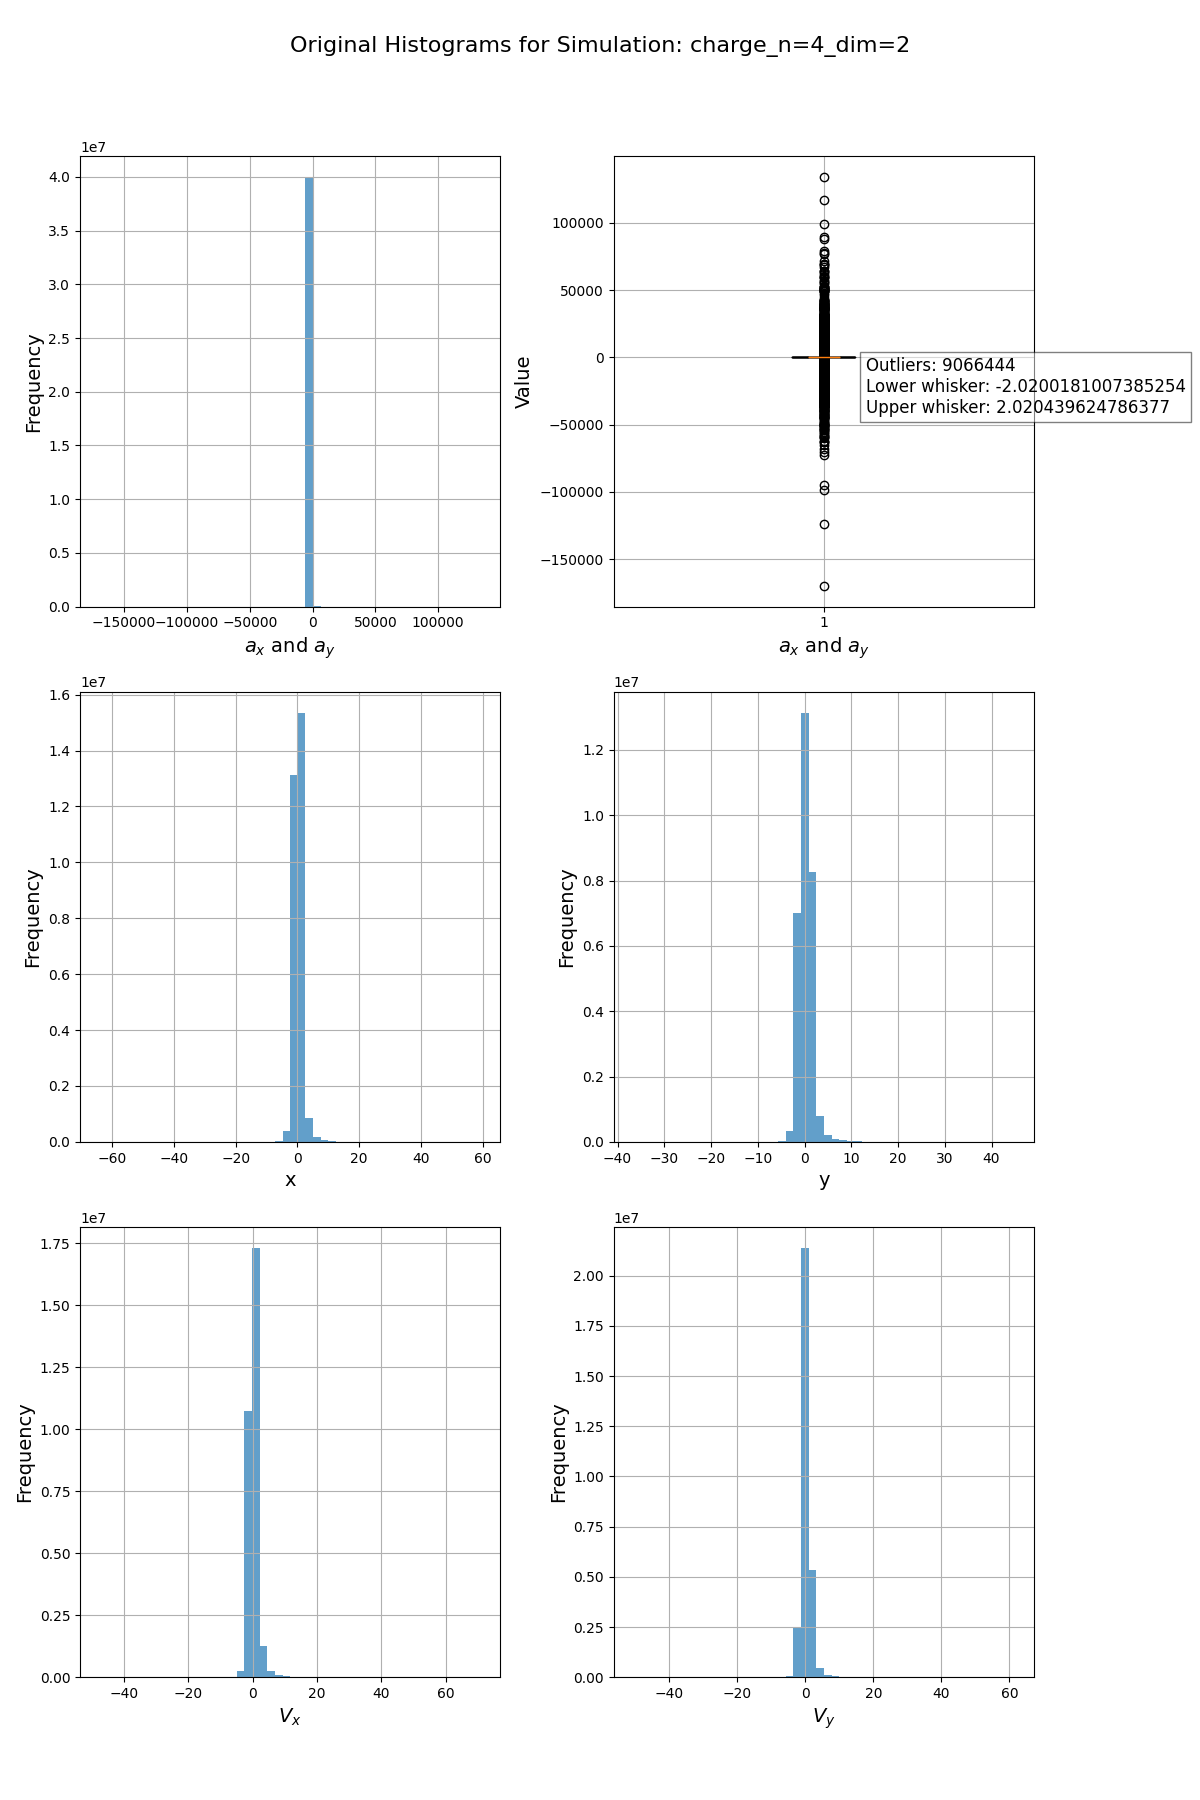
\includegraphics[width=\textwidth]{Data_Pruning/original_hist_charge_n=4_dim=2.png}
    \caption{Histograms of positional features $x$, $y$, velocity features $v_x$, $v_y$, and acceleration features $a_x$, $a_y$ for the simulated dynamical systems. The top right boxplot shows the distribution of acceleration values, highlighting the presence of outliers.}
    \label{fig:histogram1}
\end{figure}


The lower and upper whisker values shown in the box plot in Figure \ref{fig:histogram1} are calculated as 1.5 times the interquartile range (IQR) away from the first and third quartile respectively. For this calculation the distribution of acceleration values in both dimensions are used. Later, data points with acceleration values that fall outside of the whisker values are removed. The resulting pruned dataset distributions are shown in Figure \ref{fig:histogram2}.


\begin{figure}[H]
    \centering
    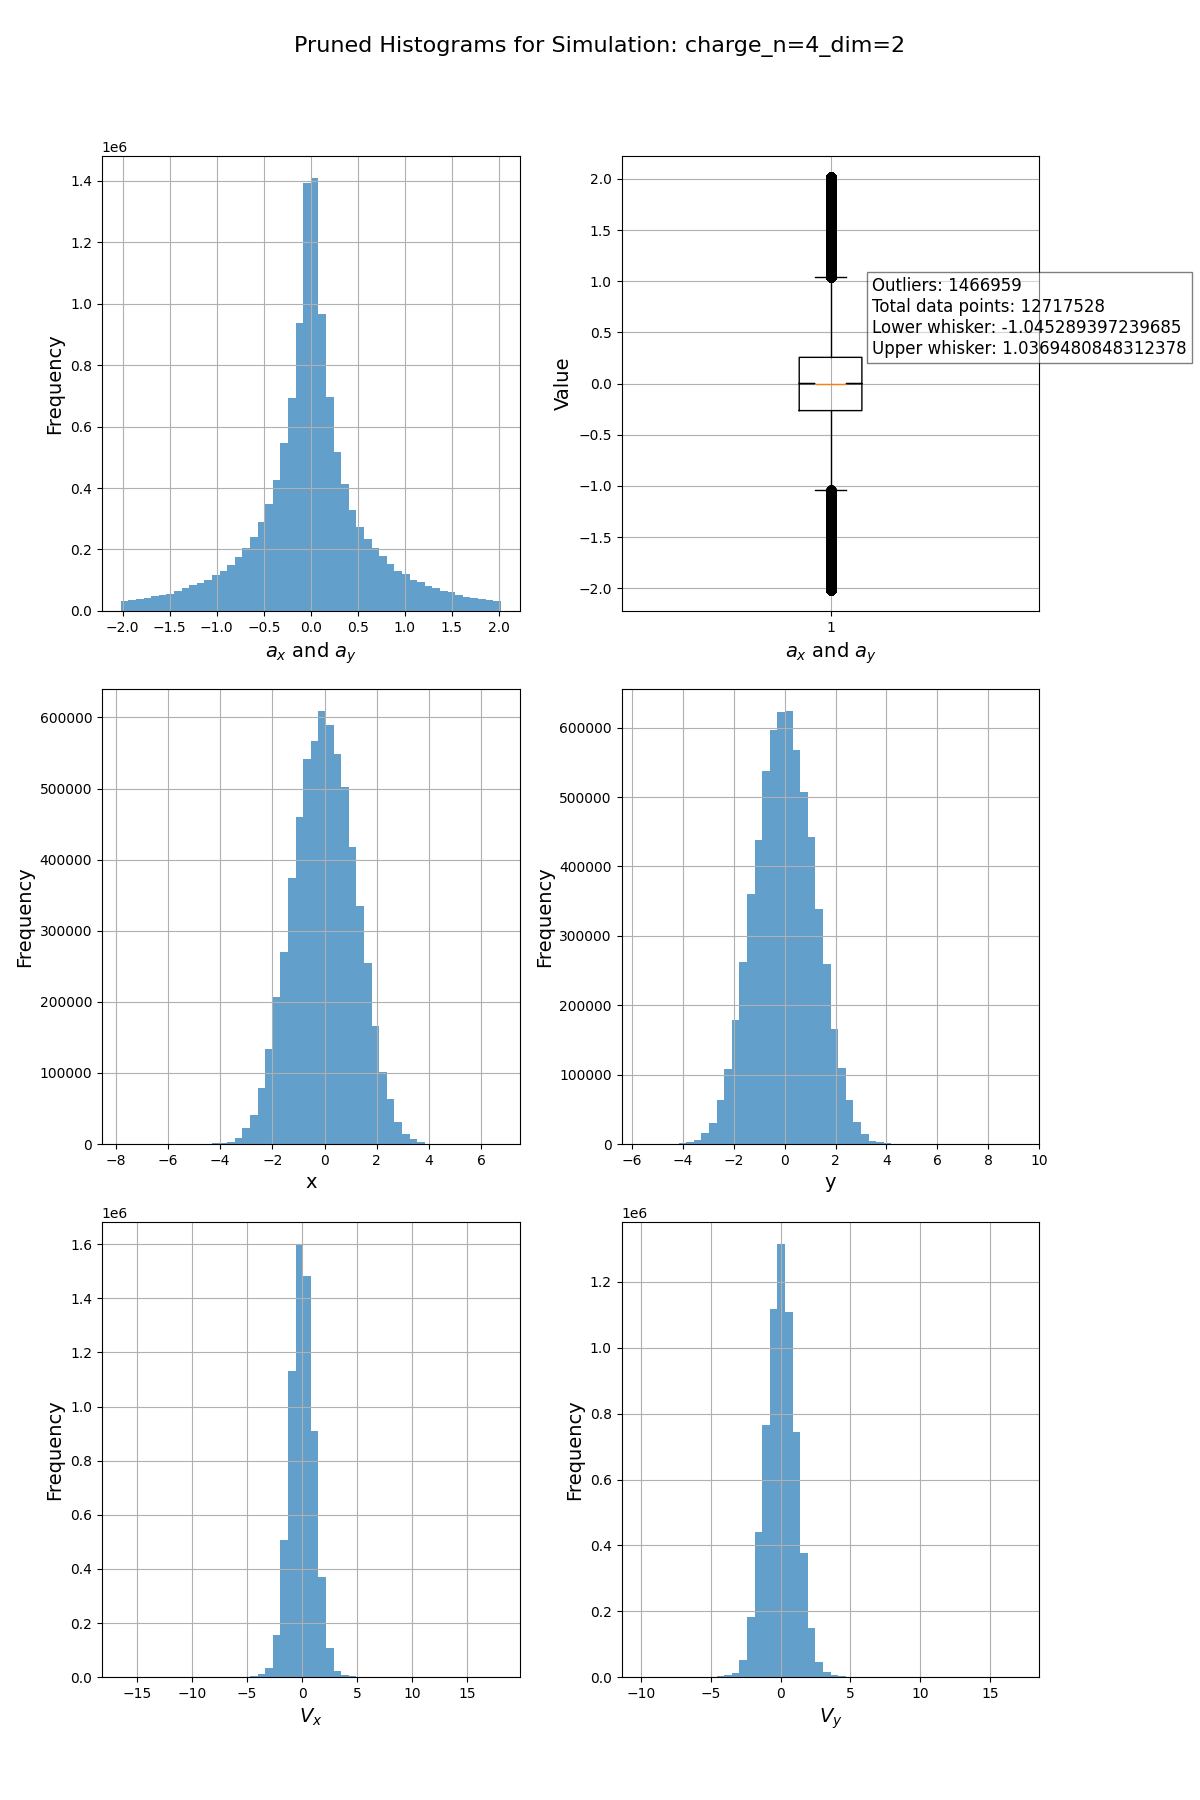
\includegraphics[width=\textwidth]{Data_Pruning/pruned_hist_charge_n=4_dim=2.png}
    \caption{Histograms of positional features $x$, $y$, velocity features $v_x$, $v_y$, and acceleration features $a_x$, $a_y$ for the pruned dataset of the simulated dynamical systems. The removal of outliers results in a more representative distribution of the typical system dynamics.}
    \label{fig:histogram2}
\end{figure}


This data pre-processing step is performed for datasets of each different dynamical systems. After the data pruning, only 1,000,000 graphs are selected for each system to ensure data pruning results in equal number of data for all systems. This number of data is later intrinsically increased by data augmentation during the training process to ensure the robustness of the model by introducing randomness in the training dataset.


\section{Models}


The GN used for the study is depicted in Figure \ref{fig:gn}.

\begin{figure}[H]
    \centering
    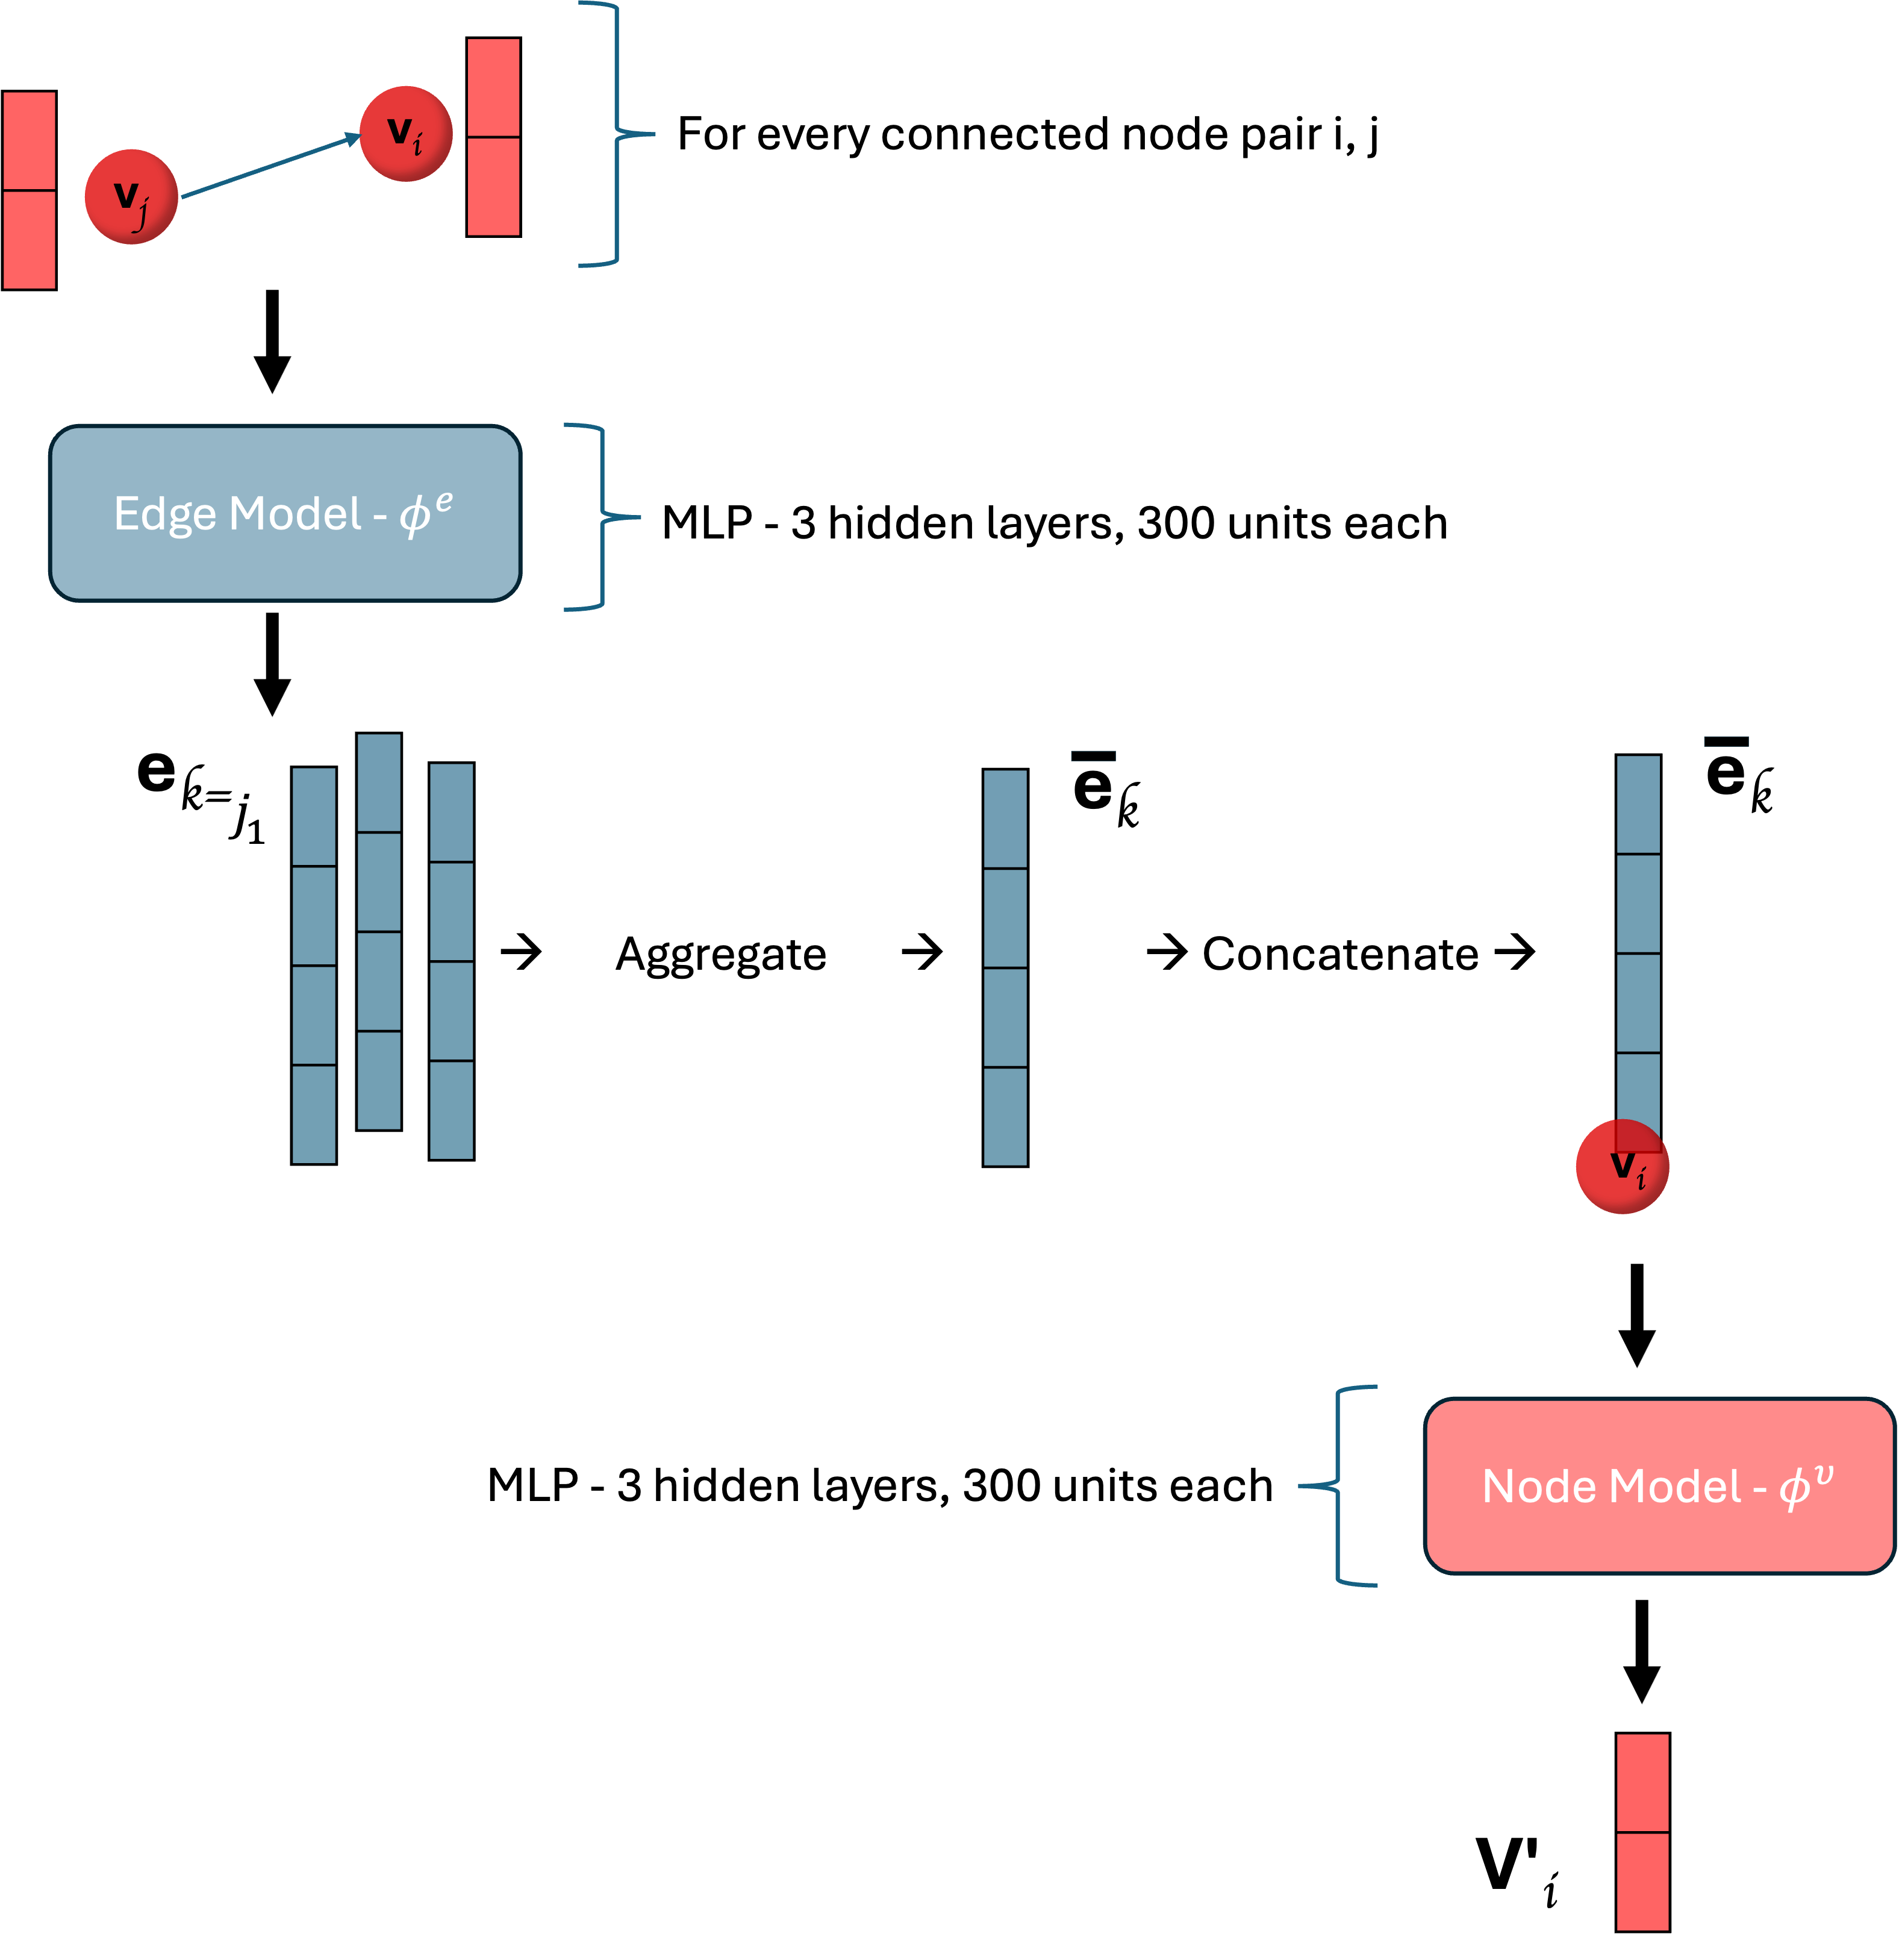
\includegraphics[width=\textwidth]{images/model.png}
    \caption{GN used for the study.}
    \label{fig:gn}
\end{figure}

The sparsity of the learned edge embeddings is introduced by adding a regularization term to the total loss function. Two different regularization methods are used in this study. The first one is the Kullback-Leibler Divergence (KL) and the second one is the L1 regularization. They are both implicity encouraging the model to learn a sparse representation of the learned messages that has the same dimension as the true number of dimension. These methods are explained below:

\subsection{Kullback-Leibler Divergence}
This model treats the message embeddings as a multinomial Gaussian distribution over the latent space and regularizes the model to minimize the KL divergence between the learned distribution and a unit normal distribution. In this case, the edge model will be designed to predict the distribution parameters: mean $\mu$ and standard deviation $\sigma$ of the normal distribution. Hence, the number of edge model outputs is increased from 100 to 200 so that the first half of the outputs predicts the means and the second half predicts the log-variance of the normal distribution. The KL-divergence term for the message regularization in the loss is:

\begin{equation}
\mathcal{L}_e = \frac{1}{N_e} \sum_{k=\{1:N_e\}} \sum_{j=\{1:L_e/2\}} \frac{1}{2} \left( \mu_{k,j}^2 + \sigma_{k,j}^2 - \log \left( \sigma_{k,j}^2 \right) \right),
\end{equation}


The \( \mu_{k,j} \) is set to be the first 100 dimensions of the edge model outputs and \( \sigma_{k,j}^2 \) is set to be the second 100 dimensions of the edge model outputs. The strength \(\alpha_1\) is set to be $10^{-2}$.


\subsection{L1 Regularization}
Formula


A bottleneck model is also used to explicitly constrain the output dimension of the edge model to the true number of dimensions. In this way, stochastically learned laten space biased by regularizer is not  

\subsection{Bottleneck Model}
Formula

\subsection{Standard Model}
No regularizations or constraints



\section{Methodology} 

The models are trained using mini-batch gradient descent with the Adam optimizer. A learning rate scheduler is employed, starting with a lower rate, gradually increasing to a maximum, and then decreasing to a rate lower than the initial. This scheduling is implemented using the OneCycleLR policy, where the maximum learning rate is set to $1e-3$, and the final learning rate decreases by a factor of $1e5$. The weight decay for the L2 regularization on the model parameters is set to $1e-5$. The loss function is the mean squared error between the predicted and true instantaneous accelerations. The total loss for the model combining the base loss, network regularization, and L1 regularization as one of the examples of the message regularization is given in \ref{eq:total_loss}.

\begin{equation}
\begin{aligned}
\mathcal{L} &= \mathcal{L}_v + \alpha_1 \mathcal{L}_e + \alpha_2 \mathcal{L}_n, \\
\mathcal{L}_v &= \frac{1}{N_v} \sum_{i \in \{1:N_v\}} \left| v_i' - \hat{v}_i' \right|, \\
\mathcal{L}_e &= \frac{1}{N_e} \sum_{k \in \{1:N_e\}} \left| e_k \right|, \\
\mathcal{L}_n &= \sum_{l \in \{1:N_l\}} \left| w_l \right|^2, \\
\alpha_1 &= 10^{-2}, \quad \alpha_2 = 10^{-8}
\end{aligned}
\end{equation}



Note that the $\mathcal{L}_e$ term is $0$ for the bottleneck and standard models, and defined as \ref{eq:KL} for the KL model.

Explain the genetic algorithm used with which imput parameters and number of iterations.

Specify/justify the choice of hyperparameters - should be the same as the paper for reproduction. But why did I choose larger L1 message coefficient (1e-2 didn't ensure sparsity)?

Explain the choice of linear, triangle or constant L1 regularization constants. 


\section{Experiments and Results}

\begin{enumerate}
    \item Table of different models loss with different regularization, just like in the table
    \item Can show the train/test loss curves over the epochs but can put in Appendix
    \item Sparsity of learned messages after training the model. Show that the number of the most variant components is equal to the dimension of the system.
    \item Linear combination of true forces vs message embeddings scatter plot along with the y-x line.
    \item R2 values table of fit of the linear combination of true forces to the learned message embeddings.
    \item Symbolic equations recovered from PySR fits.
    \item Maybe compare the symbolic equation parameters to the linear combination fits.
    \item If time left, apply symbolic regression to only simulation outputs and show that within the same iteration number the equation recovered is not correct or less accurate compared to fit to the GN latent representation.
\end{enumerate}

 
\begin{table}[h]
    \centering
\begin{tabular}{@{}lcccc@{}}
    \toprule
        Sim. &         Standard &                Bottleneck &                   L$_1$-Linear       &                   KL      \\ \midrule
    Charge-2 &           0.016  &                   0.947   &                   0.810       &                 0.185     \\                                      
    $r^{-1}$-2 &         0.000  &                   1.000   &                   0.550       &                 0.796     \\                                
    $r^{-2}$-2 &         0.004  &                   0.993   &                   0.530       &                 0.770     \\                                
    Spring-2 &           0.032  &                   1.000   &                   0.970       &                 0.883     \\ \bottomrule\\
\end{tabular}
\caption{The average $R^2$ value of a fit of
    a linear combination of true force components to the message components
    for a given model (see text) across two dimensions.
    Numbers close to 1 indicate the messages and true force are strongly correlated.
    Successes/failures of force law symbolic regression are tabled in the appendix.
    }
\label{tbl:forcefit}
\end{table}

\begin{table}[h]
    \centering
\begin{tabular}{@{}lccc@{}}
    \toprule
        Sim. & L$_1$-Constant & L$_1$-Linear & L$_1$-Triangle \\ \midrule
    Charge-2 & 0.800 & \textbf{0.810} & 0.800 \\                                      
    $r^{-1}$-2 & 0.545 & \textbf{0.550} & 0.500 \\                                
    $r^{-2}$-2 & \textbf{0.545} & 0.530 & 0.410 \\                                
    Spring-2 & 0.850 & \textbf{0.970} & 0.840 \\ \bottomrule\\
\end{tabular}
\caption{The average $R^2$ value of a fit of
    a linear combination of true force components to the message components
    for different L$_1$ regularization schedules, applied on pruned data values across two dimensions.
    Numbers close to 1 indicate the messages and true force are strongly correlated.
    }
\label{tbl:l1_schedules}
\end{table}


The test loss of each model trained on each simulation set
is given in \cref{tbl:losses}.
\begin{table*}[h]
\centering
\begin{tabular}{@{}lccccc@{}}
\toprule
Sim. & Standard & Bottleneck & L$_1$       &  KL      & FlatHGN \\ \midrule
Charge-2 & \textbf{49} & 50 & 52 & 60 & 55 \\
Charge-3 & 1.2 & 0.99 & \textbf{0.94} & 4.2 & 3.5 \\
Damped-2 & \textbf{0.30} & 0.33 & \textbf{0.30} & 1.5 & 0.35 \\
Damped-3 & 0.41 & 0.45 & \textbf{0.40} & 3.3 & 0.47 \\
Disc.-2 & 0.064 & 0.074 & \textbf{0.044} & 1.8 & 0.075 \\
Disc.-3 & 0.20 & 0.18 & \textbf{0.13} & 4.2 & 0.14 \\
$r^{-1}$-2 & 0.077 & 0.069 & 0.079 & 3.5 & \textbf{0.05} \\
$r^{-1}$-3 & 0.051 & 0.050 & 0.055 & 3.5 & \textbf{0.017} \\
$r^{-2}$-2 & 1.6 & 1.6 & \textbf{1.2} & 9.3 & 1.3 \\
$r^{-2}$-3 & 4.0 & 3.6 & 3.4 & 9.8 & \textbf{2.5} \\
Spring-2 & 0.047 & 0.046 & 0.045 & 1.7 & \textbf{0.016} \\
Spring-3 & 0.11 & 0.11 & 0.090 & 3.8 & \textbf{0.010} \\ \bottomrule
\end{tabular}
\caption{Test prediction losses for each model on each dataset in two and three
dimensions.
The training was done with the same batch size, schedule,
and number of epochs. }
\label{tbl:losses}
\end{table*}

\section{Symbolic Regression}

Symbolic Regression was performed by using the \textbf{PySR} library. Each sub-section of the GN was fit separately namely the edge model and the node model. An unseen test data of size $1000$ is passed to the GN and the outputs of the edge model and the node model are recorded. For the first symbolic fit, the predicted outputs are the most significant output features of the edge embeddings. For the L1 and standard model, this was calculated by choosing the \( n \) largest standard deviation components of the edge embeddings, where \( n \) is the true number of dimensions of the system. For the bottleneck model, this step is redundant since the edge embedding dimensions are already constrained to the true number of dimensions.


The edge model was fit to predict the mean and standard deviation of the normal distribution and the node model was fit to predict the mean and standard deviation of the normal distribution.


Show the recovered equations and discuss the symbolic generalization. MAE on training and out-of-distribution(test) set compare the trained GN performance to the symbolic equation. Eugene Wigner's article: "The language of simple, symbolic models is remarkably effective in describing the universe"


\begin{itemize}
    \item Spring, 2D, L$_1$ (expect $\phi^e_1\approx (\v{a}\cdot (\Delta x, \Delta y)) (r - 1) + b$). 
$$\phi^e_1\approx 1.36 \Delta y + 0.60 \Delta x - \frac{0.60 \Delta x + 1.37 \Delta y}{r} - 0.0025 $$
    \item $1/r^2$, 3D, Bottleneck (expect $\phi^e_1\approx \frac{\v{a}\cdot (\Delta x, \Delta y, \Delta z)}{r^3} + b$). 
$$\phi^e_1\approx \frac{0.021\Delta x m_2 - 0.077 \Delta y m_2}{r^3}$$
    \item Discontinuous, 2D, L$_1$ (expect $\phi^e_1\approx \textsc{IF}(r>2, (\v{a}\cdot (\Delta x, \Delta y, \Delta z)) r, 0) + b$). 
            $$\phi^e_1 \approx \textsc{IF}(r>2,
            0.15 r \Delta y + 0.19 r \Delta x,
            0) - 0.038$$
\end{itemize}

\section{Discussion}

\subsection{Inductive Biases}

\subsetcion{Bottleneck vs L1}

Which one performs better? Why do we choose/prefer L1? Letting the model explore a wider range of solutions without explicitly constraining the dimensionality of the edge model to the actual dimension of the system. Instead, we prefer the implicit regularization of the L1 regularization which introduces less of a bias compared to a predetermined dimensionality, and provides the flexibility of the GN to explore a wider range of solutions.


\subsection{Regularization}

Include a visual graph for linear, triangle and constant L1 regularization over epochs.

Maybe make a table for only L1 experiments: 3x4 each column is a different system, each row is a different regularization method.


Scheduler on the L1 regularization coefficient, increase the coefficient to the end max is 0.01
- Let the model explore in the beginning without huge L1 constraint, the same argument (razor) as why bottleneck doesn’t perform as well.
- There are two reasons for this, we want to increase to 1e-2 so same results but faster, the other reason is above for the schedule.

There were two motivations behind the choice of the L1 coefficient scheduler settings. The scheduler was chosen to be a linear scheduler with a start value of 0.01 and an end(maximum) value of 1. Compared to the original paper, the reason for increasing the L1 coefficient is that to encourage similar sparsity within less iteration of training. The original paper has a total training of 300 epochs whereas in this paper we choose 50 epochs for computational efficiency. The implementation of linear scheduler provies flexibility of the GN to explore a wider range of solutions in the earlier training without getting implicitly constrained by the L1 coefficient close to 1.

\subsection{Data Pruning}

In the simulated data, it was realised that some acceleration values were unusually large for xxx simulations (all except from spring). This was pruned, show histograms

\subsection{Symbolic Regression}
The details of Symbolic Regression, the loss functions used etc.

\subsection{Utilizing Computer Resources}
For this reproduction study, the Cambridge Service for Data Driven Discovery (CSD3) was utilized to train the models. The sustainability aspect of such resources were considered to make mindful choices of the use of computational resources. The training time of each model and simulated system makes up a significant part of the computational cost of this study. Hence, the total number of training epochs was limited to 100, instead of 300 as in the original paper. Considering there are 4/8 systems and 4 regularization model each to be analyzed, this reduction in training time saves 6*32 hours of single GPU node use. This consideration is both efficient for the reproduction study time and the computational cost of the study while being able to reproduce most of the results in the main paper.



\section{Conclusion}
This is an important study that uniquely shows that learned message embeddings correspond to the real force of the system (not really, but their linear combination -- hence to a linearly mapped space and mention the proof of this above).

\bibliographystyle{abbrv}
\bibliography{sample}

\appendix
\section{Generative AI}

ChatGPT 3.5 was used for suggesting alternative wordings, grammar suggestions, and proofreading while writing the report. The following prompts were used during this process

\begin{itemize}

  \item "How to represent/write \textit{[input symbol]} in LaTeX?"
  \item "What is another word for \textit{[input]} word?"
  \item "Is this sentence grammatically correct? \textit{[input sentence]}"
  \item "Is this paragraph clear for a reader? \textit{[input paragraph]}"
  \item "How to rephrase this sentence to make it more clear? \textit{[input sentence]}"
\end{itemize}


The outputs were partially adapted in a way that only alternative wordings were used and not the whole output while rephrasing the conclusion and introduction parts of the report. The LateX suggestions were used for refining the symbols and decay channel equations.

Furthermore, the suggestions from the autocomplete feature of GitHub Copilot were utilized during the documentation of the software, and code development of the project such as writing the LaTex format labels for the plots generated.



\end{document}




